\chapter{Experiments and Results}\label{ch4:experiments-results}

In this chapter, we present some quantitative and qualitative evaluations of the variants of the recreated single-view MPI model retrained on different combinations of the MannequinChallenge and RealEstate10K datasets. We use the pretrained weights of the single-view MPI model as the benchmark and compare the abilities of all model variants at hand to generate novel views. We adopt some of the quantitative metrics from Tucker and Snavely's single-view MPI paper~\cite{single_view_mpi} --- PSNR, SSMI~\cite{wang_image_2004}, and LPIPS~\cite{zhang_unreasonable_2018} --- to give numeric values to the similarities between MPI-rendered video frames and the corresponding ground truth target frames the rendering process attempts to replicate.

The model variants used to compute the metrics stated above are characterized by the following hyperparameters/metadata:
\begin{itemize}
    \item Depth loss weight, as explained in subsection~\ref{subsec:base-papers}.
    \item The number of disparity map channels specified in the \texttt{tf.function} input signature for the bilinear sampling function in our training script (Section~\ref{sec:code-sources}),\\\texttt{sample\_disparities(disparity,points)}, involving the predicted disparity and the input visible points.
    \item The lower bound on the number of visible points required per frame. Videos with even one frame having the number of visible points below this threshold would be removed from training.
    \item The choice of datasets used to train on --- MannequinChallenge, RealEstate10K, or both.
    \item Whether multiple GPU workers were engaged or not.
\end{itemize}
Even seemingly innocuous hyperparameter values such as those for the number of disparity map channels specified, we believe, could have easily held sway over training progress. Pitting these variants against each other in terms of the three computed metrics helped us select the best variant to simulate one half of a video chat with.

We manually sifted through the in-built test set of the MannequinChallenge dataset to handpick a set of 333 videos with 12,595 frames in total. These ORB-SLAM2-curated sequences had video-chat-relevant features. They mostly had the heads and torsos of people being focused on rather than there being wide shots of entire bodies. The number of people in the frames was mostly limited to one or two as opposed to there being multiple people featured. Moreover, although not a strict requirement, the head pose of people in these frames was roughly or even very loosely aligned with the camera. There was hardly anybody in any frame that seemed to look directly at the camera, such as would be expected in an actual video chat scenario. We put these cherry-picked frames in the \texttt{test-yes/} bin. We also curated \texttt{test-maybe/} (300 videos with 12,831 frames) and \texttt{test-no/} (24 videos with 728 frames) bins. They consisted of the rest of the MannequinChallenge test set with sequences either having no relevance to typical video chat settings (like there being hardly anyone in the frames) in the case of \texttt{test-no/} or falling heavily in the gray areas between \texttt{test-yes/} and \texttt{test-no/} in the case of \texttt{test-maybe/}. We even occasionally interspersed the \texttt{test-yes/} and \texttt{test-maybe/} bins with videos containing sequences that portrayed people facing diametrically opposite to the camera. This was just so we could really challenge the model variant being tested.

Of the various aspects of the code that we modelled from the textual descriptions and relevant code snippets obtained from both the single-view and stereo MPI papers such as \texttt{generator\_wandb.py}, \texttt{data\_loader.py}, \texttt{train\_wandb.py}, and \texttt{test.py}, the scripts relevant to the experiments in this section are \texttt{test.py} and\\\texttt{generator\_wandb.py} (Section~\ref{sec:code-sources}). For testing, the generator first aggregates all videos names from the directory input to it and for each of these, it picks various \texttt{reference\_image} and \texttt{target\_image} pairs which are internally 5 frames apart. \texttt{reference\_image} is the frame that \texttt{test.py} uses to infer the MPI representation of the scene from and \texttt{target\_image} is supposedly a view of the same scene from a different angle. The possibility that, when the camera moves from one scene to another in the same video, \texttt{reference\_image} may depict a scene different from the one captured by \texttt{target\_image} is expected to be extremely low as both datasets have been curated by similar ORB-SLAM2 and COLMAP processes. In such hypothetical cases, \texttt{target\_image} will be erroneously rendered by \texttt{mpi.render} function as the corresponding \texttt{rendered\_image}. But since we take the mean of the computed metrics over hundreds of \texttt{test.py} processed \texttt{reference\_image}, \texttt{target\_image} pairs, we believe the final accuracies of a variant's mean metrics will not be off the tracks much and that they shall still be used to determine a variant’s performance satisfactorily. Each of the three metrics are calculated between \texttt{target\_image} and \texttt{rendered\_image}, which are situated 5 frames apart along the camera trajectory of the respective clip. We did not repeat the same test process for frames 10 apart, which would just have done been to show (as in the case of the single-view MPI paper) that the longer the baseline between reference/source and target views, the less the accuracy will be of the rendered image. On the same note, we have also not calculated the metrics internally for all processed \texttt{(reference\_image, target\_image)} pairs, which would just have been done to catch the hypothetical anomalies of the complete scene changes mentioned before. 

We also took an interesting little detour in our project when we attempted to parallelize training across multiple GPUs, which we believed would allow us to increase the batch size\footnote{currently limited to 4 pairs of reference and target images and their respective camera poses and intrinsics, along with the 3D points of the reference image} and thereby let larger and larger parts of our 60000+ training ready sequences with associated point clouds be used for learning by our recreated model. This would have assisted the model in better avoiding local minima and maxima. But, since TensorFlow's direct conversion procedure that would let standard single-GPU-utilizing scripts become multi-GPU-faring is as yet still an evolving process requiring careful attention to resource allocation issues among the various replicas of the parallelizable aspects of the model\footnote{such as the dataset generator, the loss functions aggregator, etc.} spread across GPUs, our training got undercut after a good start by a resource exhaustion error at training step 178. Nevertheless, we computed all three metrics for this other model variant retrained on MannequinChallenge data using \texttt{tf.distribute.MirroredStrategy}, and capable of harnessing the power of multiple GPUs.

The rest of this chapter presents the results of the experiments done with the various model variants and the baseline pretrained model. We then cap it all off by presenting the results of incorporating OpenFace 2.2 into the inference pipeline. As of this writing, our generator is only able to pick random pairs of reference and target frames from the 333 \texttt{test-yes/} videos. Sequential pair-picking would avoid possible repetition of selected pairs and allow for an exhaustive coverage of the test set. Given that even the smaller of the two datasets has 100,000+ frames and that we have not been able to resolve the issue of the synthesized disparity maps becoming smudgier and smudgier until they turn completely gray/monochromatic even before any of the variants hit 14,000 training steps, it is not very likely that the model may see the same frame twice. So perhaps, computing evaluation metrics with training data can double in as doing the same with validation data itself, even though we haven't set aside validation data. As for the metrics, an LPIPS value of 0 indicates there is either a perfect match between the images being compared or the images being compared are one and the same. To the contrary, SSIM values of 1 indicate a perfect match. Both these metrics range from 0 to 1. PSNR values, measured in decibels (dB), don't generally have an upper limit but values 20 dB and higher are considered acceptable. In calibrating our implementations of these metrics, when we compared an image with itself, we found the mean LPIPS, SSIM and PSNR values over 300 images to be close to 0, 1, and 30, respectively.

\begin{figure}[!h]
    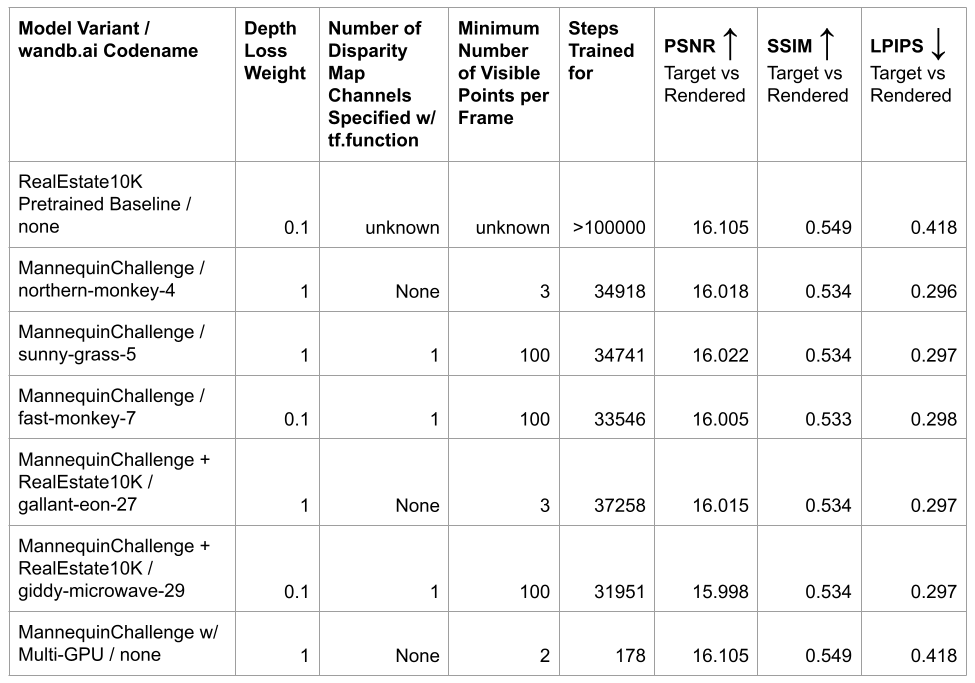
\includegraphics[width=1\columnwidth]{figures/model-variants-metrics.png}
    \caption{Model Variants' Mean PSNR, SSIM, and LPIPS Evaluation Values Over 300 Testing Instances}
    \label{fig:model-variants-metrics}
\end{figure}

We can get a sense of how the variants stack up against one another from figure~\ref{fig:model-variants-metrics}. Perceptual similarity comes the closest to the way humans judge the picture quality of an image. Hence, we chose the variant northern-monkey-4 for the final step of simulating a video chat. These interesting names are automatically allotted by wandb.ai at the start of any training run. If the run is relatively successful, we use the final model produced by it as one of our variants and evaluate its performance. All our variants have been trained to the limit and to the point where the loss becomes less than 1, after having come down all the way from 1188, and stagnates. This has always occurred sooner than 25,000 training steps for all our variants (Figure~\ref{fig:mean-loss}). It goes to show that had we been entirely successful in our implementation of the model, we would also have been able to train for way more than 100,000 steps, similarly to Tucker and Snavely~\cite{single_view_mpi}. 

\begin{figure}[!h]
    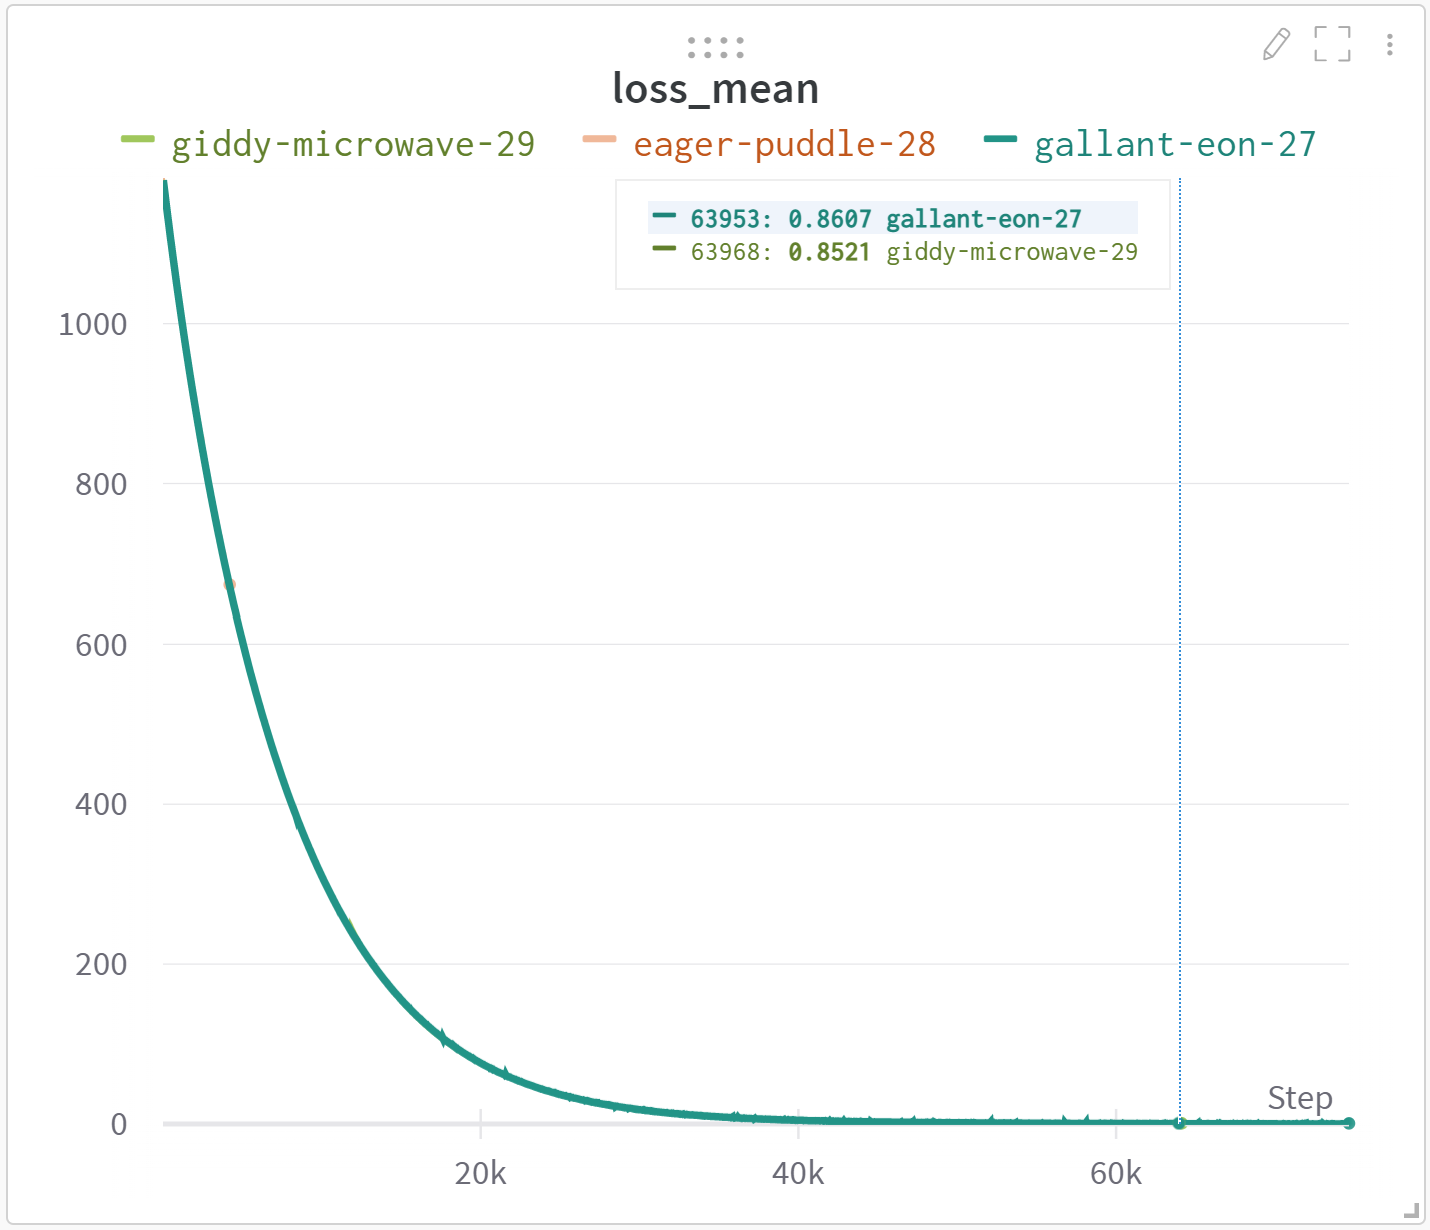
\includegraphics[width=0.75\columnwidth]{figures/mean-loss.png}
    \caption{Typical Mean Loss Chart for Any of Our Training Runs}
    \label{fig:mean-loss}
    {\small wandb.ai somehow always shows twice the number of actual training steps completed on our server. Hence all our variants' training stagnates at 30,000+ steps and not at the 60,000+ steps shown in this wandb.ai-logged loss chart.}
\end{figure}

\begin{figure}[!h]
    \begin{tabular}{cccc}

        \subfloat[]{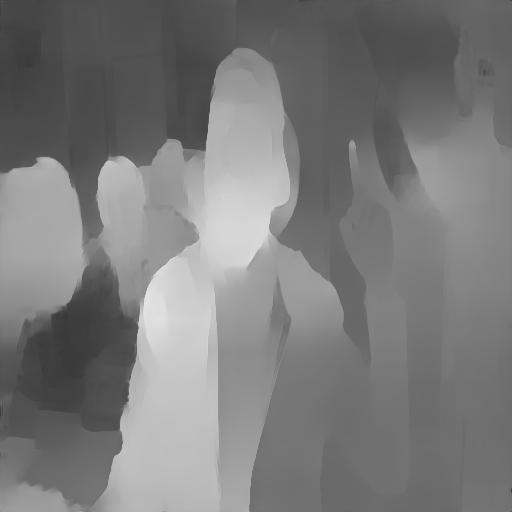
\includegraphics[width = 1.3in]{figures/baseline/000001_image_disparity.png}} &
        \subfloat[PSNR $\uparrow$ Target vs Rendered = 12.345]{\includegraphics[width = 1.3in]{figures/baseline/000001_image_reference.png}} &
        \subfloat[SSIM $\uparrow$ Target vs Rendered = 0.509]{\includegraphics[width = 1.3in]{figures/baseline/000001_image_target.png}} &
        \subfloat[LPIPS $\downarrow$ Target vs Rendered = 0.520]{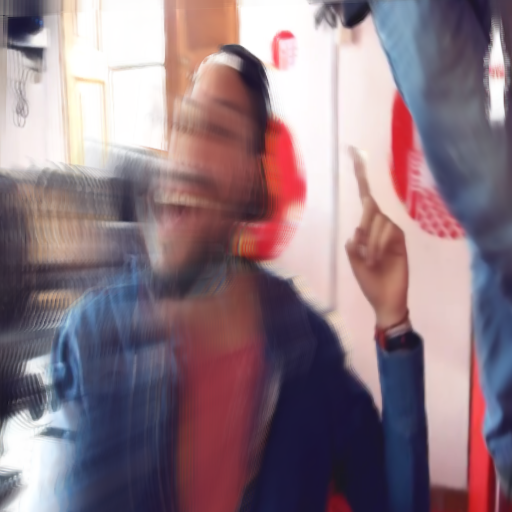
\includegraphics[width = 1.3in]{figures/baseline/000001_image_render.png}}\\
        
        \subfloat[]{
\includegraphics[width = 1.3in]{figures/gallant-eon-27/000001_image_disparity.png}} &
        \subfloat[PSNR $\uparrow$ Target vs Rendered = 12.300]{\includegraphics[width = 1.3in]{figures/gallant-eon-27/000001_image_reference.png}} &
        \subfloat[SSIM $\uparrow$ Target vs Rendered = 0.470]{\includegraphics[width = 1.3in]{figures/gallant-eon-27/000001_image_target.png}} &
        \subfloat[LPIPS $\downarrow$ Target vs Rendered = 0.338]{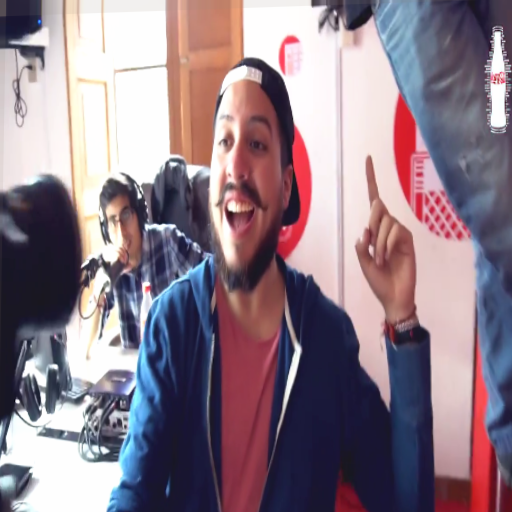
\includegraphics[width = 1.3in]{figures/gallant-eon-27/000001_image_render.png}}\\
        
        \subfloat[]{
\includegraphics[width = 1.3in]{figures/giddy-microwave-29/000001_image_disparity.png}} &
        \subfloat[PSNR $\uparrow$ Target vs Rendered = 12.282]{\includegraphics[width = 1.3in]{figures/giddy-microwave-29/000001_image_reference.png}} &
        \subfloat[SSIM $\uparrow$ Target vs Rendered = 0.470]{\includegraphics[width = 1.3in]{figures/giddy-microwave-29/000001_image_target.png}} &
        \subfloat[LPIPS $\downarrow$ Target vs Rendered = 0.338]{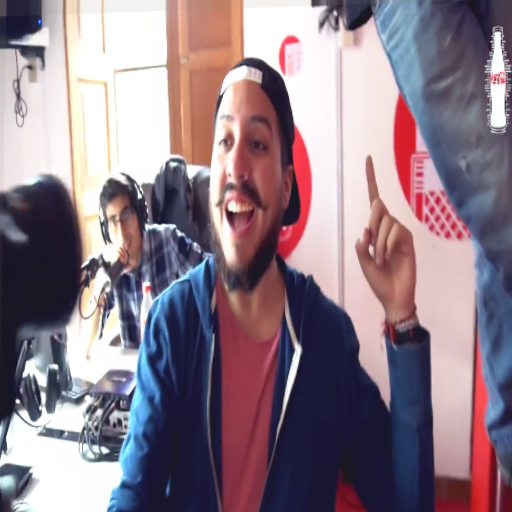
\includegraphics[width = 1.3in]{figures/giddy-microwave-29/000001_image_render.png}}

    \end{tabular}
    \caption{Baseline and (MannequinChallenge+RealEstate10K)-Based Model Variants' Output Visualizations With a MannequinChallenge Target Frame}
    \label{fig:output-visualizations-1}
    {\small Variants from top to bottom: baseline, gallant-eon-27, giddy-microwave-29\\Outputs from left to right: disparity map, reference frame, target frame, rerendered target}
\end{figure}

What further validates our choice of northern-monkey-4 is the set of output visualizations for all relatively successful model variants shown in figures~\ref{fig:output-visualizations-1} and~\ref{fig:output-visualizations-2}. These outputs further reveal that even prior to all our fine-tuning the pretrained model found it hard to synthesize the disparity for video-chat-relevant frames. In the testing example used, the person has clearly moved closer to the camera but the frame synthesized by the baseline model shows ``stack of cards" effects. This could potentially also be the reason that while the picture quality for the renderings seems to have been greatly improved by our fine-tuning (evident from the improved LPIPS values), the already nebulous disparity synthesis (when it comes to video chat frames) has been rendered asunder. It also stands to reason that perhaps depth/disparity is taken more into account by the SSIM metric than the other two metrics, owing to the stark decrease in SSIM values for the fine-tuned variants. It is structural similarity after all, and we have already established that depth is part of the 3D structure of the scene. Hence, we have also been further validated in our efforts to even stick to the course of retraining the baseline model in the first place.

\begin{figure}[!h]
    \begin{tabular}{cccc}

        \subfloat[]{
\includegraphics[width = 1.3in]{figures/northern-monkey-4/000001_image_disparity.png}} &
        \subfloat[PSNR $\uparrow$ Target vs Rendered = 12.315]{\includegraphics[width = 1.3in]{figures/northern-monkey-4/000001_image_reference.png}} &
        \subfloat[SSIM $\uparrow$ Target vs Rendered = 0.470]{\includegraphics[width = 1.3in]{figures/northern-monkey-4/000001_image_target.png}} &
        \subfloat[LPIPS $\downarrow$ Target vs Rendered = 0.337]{\includegraphics[width = 1.3in]{figures/northern-monkey-4/000001_image_render.png}}\\
        
        \subfloat[]{
\includegraphics[width = 1.3in]{figures/sunny-grass-5/000001_image_disparity.png}} &
        \subfloat[PSNR $\uparrow$ Target vs Rendered = 12.315]{\includegraphics[width = 1.3in]{figures/sunny-grass-5/000001_image_reference.png}} &
        \subfloat[SSIM $\uparrow$ Target vs Rendered = 0.470]{\includegraphics[width = 1.3in]{figures/sunny-grass-5/000001_image_target.png}} &
        \subfloat[LPIPS $\downarrow$ Target vs Rendered = 0.337]{\includegraphics[width = 1.3in]{figures/sunny-grass-5/000001_image_render.png}}\\
        
        \subfloat[]{
\includegraphics[width = 1.3in]{figures/fast-monkey-7/000001_image_disparity.png}} &
        \subfloat[PSNR $\uparrow$ Target vs Rendered = 12.284]{\includegraphics[width = 1.3in]{figures/fast-monkey-7/000001_image_reference.png}} &
        \subfloat[SSIM $\uparrow$ Target vs Rendered = 0.471]{\includegraphics[width = 1.3in]{figures/fast-monkey-7/000001_image_target.png}} &
        \subfloat[LPIPS $\downarrow$ Target vs Rendered = 0.339]{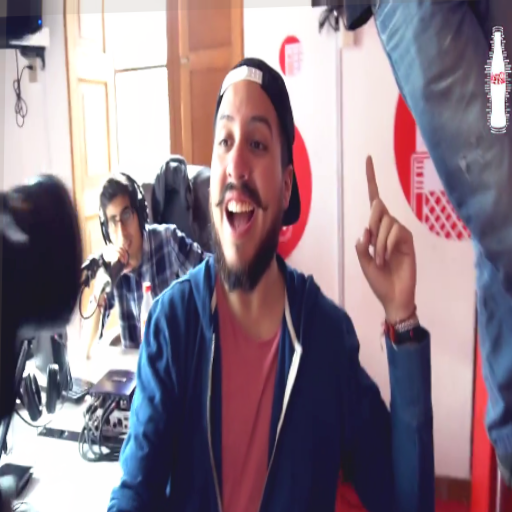
\includegraphics[width = 1.3in]{figures/fast-monkey-7/000001_image_render.png}}\\

    \end{tabular}
    \caption{MannequinChallenge-Based Model Variants' Output Visualizations With a MannequinChallenge Target Frame}
    \label{fig:output-visualizations-2}
    {\small Variants from top to bottom: northern-monkey-4, sunny-grass-5, fast-monkey-7\\Outputs from left to right: disparity map, reference frame, target frame, rerendered target}
\end{figure}

In reference to the qualitative results presented throughout this work, we invoke the reader to adopt Tucker and Snavely's~\cite{single_view_mpi} use of pointers such as the handling of occluded content, the production of undesirable artifacts at the edges of foreground objects, and so on, to qualitatively compare the discrepancies in the results generated by each model variant. Similarly, visually checking for the accuracy of the synthesized disparity maps, as was illustrated at the beginning of chapter~\ref{ch3:methods}, is also useful in verifying the quality of the MPIs produced. We encourage the reader to zoom into the electronic version of this thesis or take to the GitHub repository accompanying this work (Section~\ref{sec:code-sources}) for easier visual verification.


% To cap it off with the help of OpenFace 2.2, we also include a few snapshots of how a rerendered frames vary with changes in head pose in figure~\ref{fig:rerendered-with-openface}.  

% As the girl looks to the left the opposite concurrent video frame moves to the right and vice versa
% Please head over to the github repo for this project to observe videos of simultaneous changes simulating a two way video chat.
% testing bring testing to sequential process instead or random using hid generator code

